\chapter{Analisi concettuale del sistema}

In questo capitolo verrano mostrati gli aspetti delo sviluppo della piattaforma per quanto riguarda il progetto della base di dati.\cite{DB}

\section{Analisi dei requisiti}

Per progettare una base di dati è necessario comprendere la realtà da rappresentare effettuando la cosiddetta raccolta dei requisiti, cioè l'individuazione dei problemi che l'applicazione deve risolvere tenendo presenti sia gli aspetti statici (i dati) che quelli dinamici (le operazioni sui dati).\\

Segue un elenco dei requisiti della base di dati per lo specifico sistema informatico. 

\hangindent=1cm
\hangafter=1
{\scshape I giocatori.} Di ogni giocatore interessa l'email (che deve essere unica), l'username, la password se effettua il login standard, il provider se effettua il login con OAuth e il ruolo che gli è stato assegnato. Ogni giocatore può seguire o essere seguito da altri giocatori. Ogni giocatore può pubblicare dei giochi, può pubblicare recensioni, votare positivamente o negativamente e aggiungere ad una lista preferiti dei giochi. Per il servizio typingDNA è necessario inoltre conoscere il numero di login effettuati, se il giocatore è stato registrato nel sistema di typingDNA e quanti tentativi ha a disposizione prima che gli venga bloccato l'account.

\hangindent=1cm
\hangafter=1
{\scshape I giochi.} Di ogni gioco interessa il titolo, la descrizione, la categoria, l'utente che l'ha pubblicato e opzionalmente la versione. Ogni gioco è composto da un solo blocco di file di build. I giochi possono essere recensiti, votati e resi preferiti da più giocatori contemporaneamente.

\hangindent=1cm
\hangafter=1
{\scshape I file di build} sono un blocco composto da 5 file specifici del framework Unity con il quale i giochi devono essere programmati per poter funzionare sulla piattaforma.

\hangindent=1cm
\hangafter=1
{\scshape Le recensioni.} Di ogni recensione interessa la data di pubblicazione, il testo, l'utente che l'ha pubblicata e il gioco a cui si riferisce.

\section{La progettazione concettuale}
Lo scopo della progettazione concettuale è quello di rappresentare le specifiche informali ricavabili dai requisiti in modo schematico. Questo schema prende il nome di schema ER (Entità-Relazione). Si tratta di un modello concettuale ad alto livello di astrazione che, quindi, non tiene conto degli aspetti implementativi.

\subsection{Lo schema Entità-Relazione}
Oltre allo schema ER è necessario riportare delle tabelle descrittive per le entità, relazioni e attributi.


\begin{table}[hbt!]
    \centering
    \begin{tabular}{ m{0.15\textwidth} m{0.24\textwidth} m{0.24\textwidth} m{0.24\textwidth} }
        \hline
        \textbf{Entità} & \textbf{Descrizione} & \textbf{Attributi} & \textbf{Identificatori} \\
        \hline
        \textbf{Giocatore} & Utente registrato nell'applicazione & email, password, provider, ruolo, numero di login, registrato su typingDNA, tentativi typingDNA & \{email\} \\
        \hline
        \textbf{Gioco} & Gioco caricato sulla piattaforma & game id, titolo, descrizione, categoria, versione & \{game id\} \\
        \hline
        \textbf{Recensione} & Recensione pubblicata da un giocatore per un gioco & data, testo & \{giocatore, gioco\} \\
        \hline
        \textbf{File di build} & Blocco di file di build di un gioco &  & \{gioco\} \\
        \hline
        \textbf{File} & Il singolo file di build & file id, nome, contenuto & \{file id\} \\
    \end{tabular}
    \caption{Entità}
\end{table}

\begin{table}[hbt!]
    \centering
    \begin{tabular}{ m{0.17\textwidth} m{0.18\textwidth} m{0.18\textwidth} m{0.18\textwidth} m{0.18\textwidth} }
        \hline
        \textbf{Relazione} & \textbf{Descrizione} & \textbf{Componenti} & \textbf{Attributi} & \textbf{Identificatori} \\
        \hline
        \textbf{Pubblicazione} & Ogni gioco è pubblicato da un utente & Giocatore\newline Gioco & data & \{gioco\} \\
        \hline
        \textbf{Pubblica} & Un giocatore può pubblicare una recensione & Giocatore\newline Recensione &  & \{recensione\} \\
        \hline
        \textbf{RG} & Ogni recensione è legata ad un gioco & Recensione\newline Gioco & & \{recensione\} \\
        \hline
        \textbf{Preferito} & Un giocatore può aggiungere un gioco ai suoi preferiti & Giocatore\newline Gioco & & \{giocatore, gioco\} \\
        \hline
        \textbf{Relazione} & Un giocatore può seguirne un altro & Giocatore\newline Giocatore & & \{seguace, seguito\} \\
        \hline
        \textbf{Voto} & Voto espresso da un giocatore per un gioco & Giocatore\newline Gioco & valore & \{giocatore, gioco\} \\
        \hline
        \textbf{Composto da} & Un gioco può avere allegato un blocco di file & Gioco\newline File di build & & \{file di build\} \\
        \hline
        \textbf{Comprende} & Ogni blocco di file di build è composto da 5 file & File di build\newline File &  & \{file\} \\
    \end{tabular}
    \caption{Relazioni}
\end{table}

\begin{table}[hbt!]
    \centering
    \begin{tabular}{m{0.18\textwidth} m{0.24\textwidth} m{0.19\textwidth} m{0.32\textwidth}}
        \hline
        \textbf{Attributo} & \textbf{Entità/Relazione} & \textbf{Dominio} & \textbf{Descrizione} \\
        \hline
        \textbf{Email} & Giocatore & String & L'email del giocatore \\
        \hline
        \textbf{Ruolo} & Giocatore & String & Il ruolo del giocatore nell'applicazione \\
        \hline
        \textbf{Numero di login} & Giocatore & Integer & Numero di accessi al sito per il giocatore \\
        \hline
        \textbf{Registrato su typingDNA} & Giocatore & Boolean & Un giocatore è registrato su typingDNA quando ha fatto vari login sulla piattaforma \\
        \hline
        \textbf{Tentativi typingDNA} & Giocatore & Integer & Numero di tentativi di autenticazione con typingDNA \\
        \hline
        \textbf{Password} & Giocatore & String & La password per accedere con il proprio account \\
        \hline
        \textbf{Provider} & Giocatore & String & Il provider del servizio OAuth per il giocatore \\
        \hline
        \textbf{Data} & Pubblicazione & Date & La data di pubblicazione di un gioco \\
        \hline
        \textbf{Data} & Recensione & Date & La data di pubblicazione di una recensione  \\
        \hline
        \textbf{Testo} & Recensione & Text & Testo di una recensione \\
        \hline
        \textbf{Valore} & Voto & Integer & Voto dato ad un gioco. Può essere +1 o -1 \\
        \hline
        \textbf{Game ID} & Gioco & Integer & Numero identificativo di un gioco \\
        \hline
        \textbf{Titolo} & Gioco & String & Titolo di un gioco \\
        \hline
        \textbf{Descrizione} & Gioco & Text & Descrizione di un gioco \\
        \hline
        \textbf{Categoria} & Gioco & String & La categoria di cui fa parte un gioco \\
        \hline
        \textbf{Versione} & Gioco & String & La versione di patch di un gioco \\
        \hline
        \textbf{File ID} & File & Integer & Numero che identifica un file \\
        \hline
        \textbf{Nome} & File & String & Nome del file \\
        \hline
        \textbf{Contenuto} & File & BLOB & Contenuto effettivo del file che permette l'esecuzione del gioco \\
    \end{tabular}
    \caption{Attributi}
\end{table}

\begin{figure}[hbt!]
    \centering
    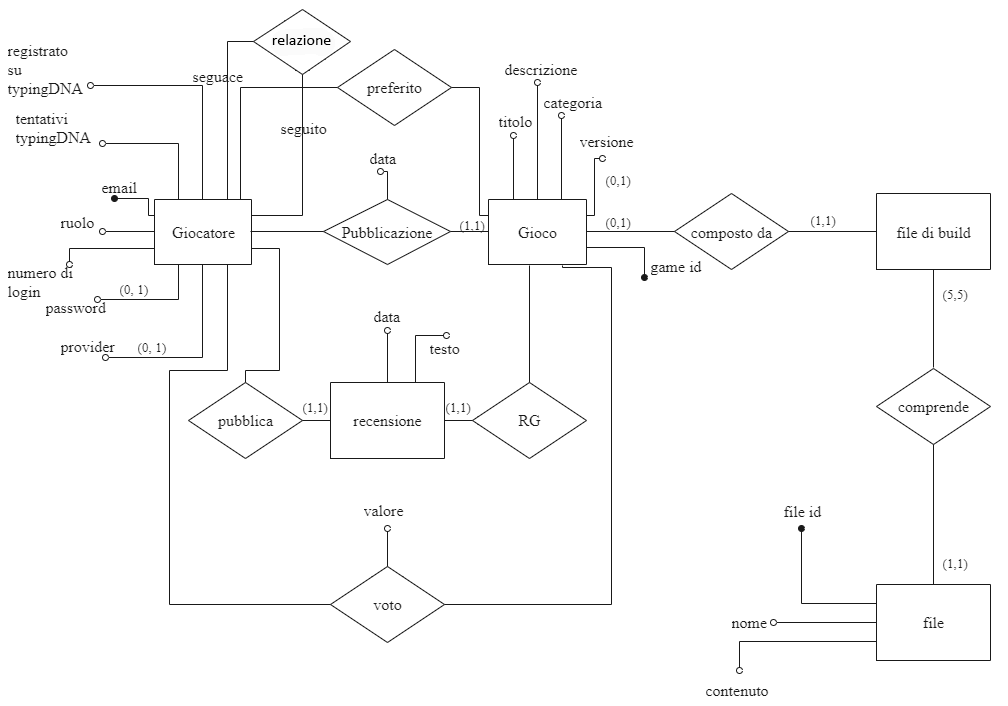
\includegraphics[angle=-90, width=\textwidth]{schemaER}
    \caption{Schema ER}
\end{figure}

\begin{table}[hbt!]
    \centering
    \begin{tabular}{m{0.18\textwidth} m{0.24\textwidth} m{0.55\textwidth}}
        \hline
        \textbf{Relazione} & \textbf{Componenti} & \textbf{Vincoli di cardinalità}\\ \hline
        \textbf{Relazione} & Seguace & Ogni giocatore può essere seguace di 0 o più giocatori \\ \cline{2-3}
        & Seguito & Ogni giocatore può essere seguito da 0 o più giocatori \\ \hline
        \textbf{Pubblicazione} & Giocatore & Ogni giocatore può pubblicare 0 o più giochi \\ \cline{2-3}
        & Gioco & Ogni gioco è pubblicato da uno e un solo giocatore \\ \hline
        \textbf{Pubblica} & Giocatore & Ogni giocatore può pubblicare 0 o più recensioni \\ \cline{2-3}
        & Recensione & Ogni recensione è pubblicata da uno e un solo giocatore \\ \hline
        \textbf{RG} & Recensione & Ogni recensione appartiene ad uno e un solo gioco \\ \cline{2-3}
        & Gioco & Ogni gioco può avere 0 o più recensioni \\ \hline
        \textbf{Voto} & Giocatore & Ogni giocatore può esprimere 0 o più voti \\ \cline{2-3}
        & Gioco & Ogni gioco può ricevere 0 o più voti \\ \hline
        \textbf{Preferito} & Giocatore & Ogni giocatore può aggiungere ai preferiti 0 o più giochi \\ \cline{2-3}
        & Gioco & Ogni gioco può essere preferito da 0 o più giocatori \\ \hline
        \textbf{Composto da} & Gioco & Ogni gioco ha allegato 0 o un blocco di file \\ \cline{2-3}
        & File di build & Ogni blocco di file di build è legato ad uno e un solo gioco \\ \hline
        \textbf{Comprende} & File di build & Ogni blocco di file di build è costituito da 5 file \\ \cline{2-3}
        & File & Ogni file appartiene ad un solo blocco di file di build \\
    \end{tabular}
    \caption{Vincoli di cardinalità}
\end{table}

\FloatBarrier
\subsection{Le \emph{business rules}}
Lo schema ER è fondamentale per comprendere la struttura astratta dell'applicazione, ma ha dei limiti. Non tutte le problematiche sono codificabili con questo schema e perciò è necessario aggiungere dei vincoli esterni (spesso chiamati \emph{business rules}) che lo completano.

\begin{table}[hbt!]
    \begin{tabular}{p{1cm} m{0.88\textwidth}}
        \hline
        & \textbf{Vincoli d'integrità non esprimibili nel diagramma ER} \\
        \hline 
        \textbf{1} & Ogni istanza di Giocatore non può partecipare contemporaneamente alla stessa istanza di following con il ruolo di Seguito e Seguace. \\ \hline
        \textbf{2} & Per ogni istanza di Giocatore, almeno uno tra i campi \emph{password} e \emph{provider} deve essere presente. Se \emph{provider} è presente allora anche \emph{password} deve esserlo \\ \hline
        \textbf{3} & Per ogni istanza di Giocatore, il campo \emph{ruolo} può assumere solo i seguenti valori: \emph{player, moderator, admin}. \\ \hline
        \textbf{4} & Per ogni istanza di Voto, il campo \emph{valore} può essere solo -1 o +1. \\ \hline
        \textbf{5} & Per ogni istanza di Gioco, il campo \emph{versione}, se presente, deve avere il seguente formato: \emph{Integer.Integer.Integer}. \\ \hline
        \textbf{6} & Per ogni istanza di Iscritto OAuth, il campo \emph{provider} può essere solo \emph{google} o \emph{github}. \\ \hline
        \textbf{7} & Per ogni istanza di Gioco, il campo \emph{categoria} può assumere solo i seguenti valori: \emph{Action, Adventure, Casual, Indie, Racing, RPG, Simulation, Sports, Strategy, Other}. \\ \hline
        \textbf{8} & Per ogni istanza di Giocatore, i campi \emph{tentativi typingDNA, numero di login} devono essere $\geq$ 0. \\
    \end{tabular}
    \caption{Vincoli esterni}
\end{table}